\section{The \fermi Gamma-ray Space Telescope}
\seclabel{fermi_telescope}

\begin{figure}[htbp]
  \centering
  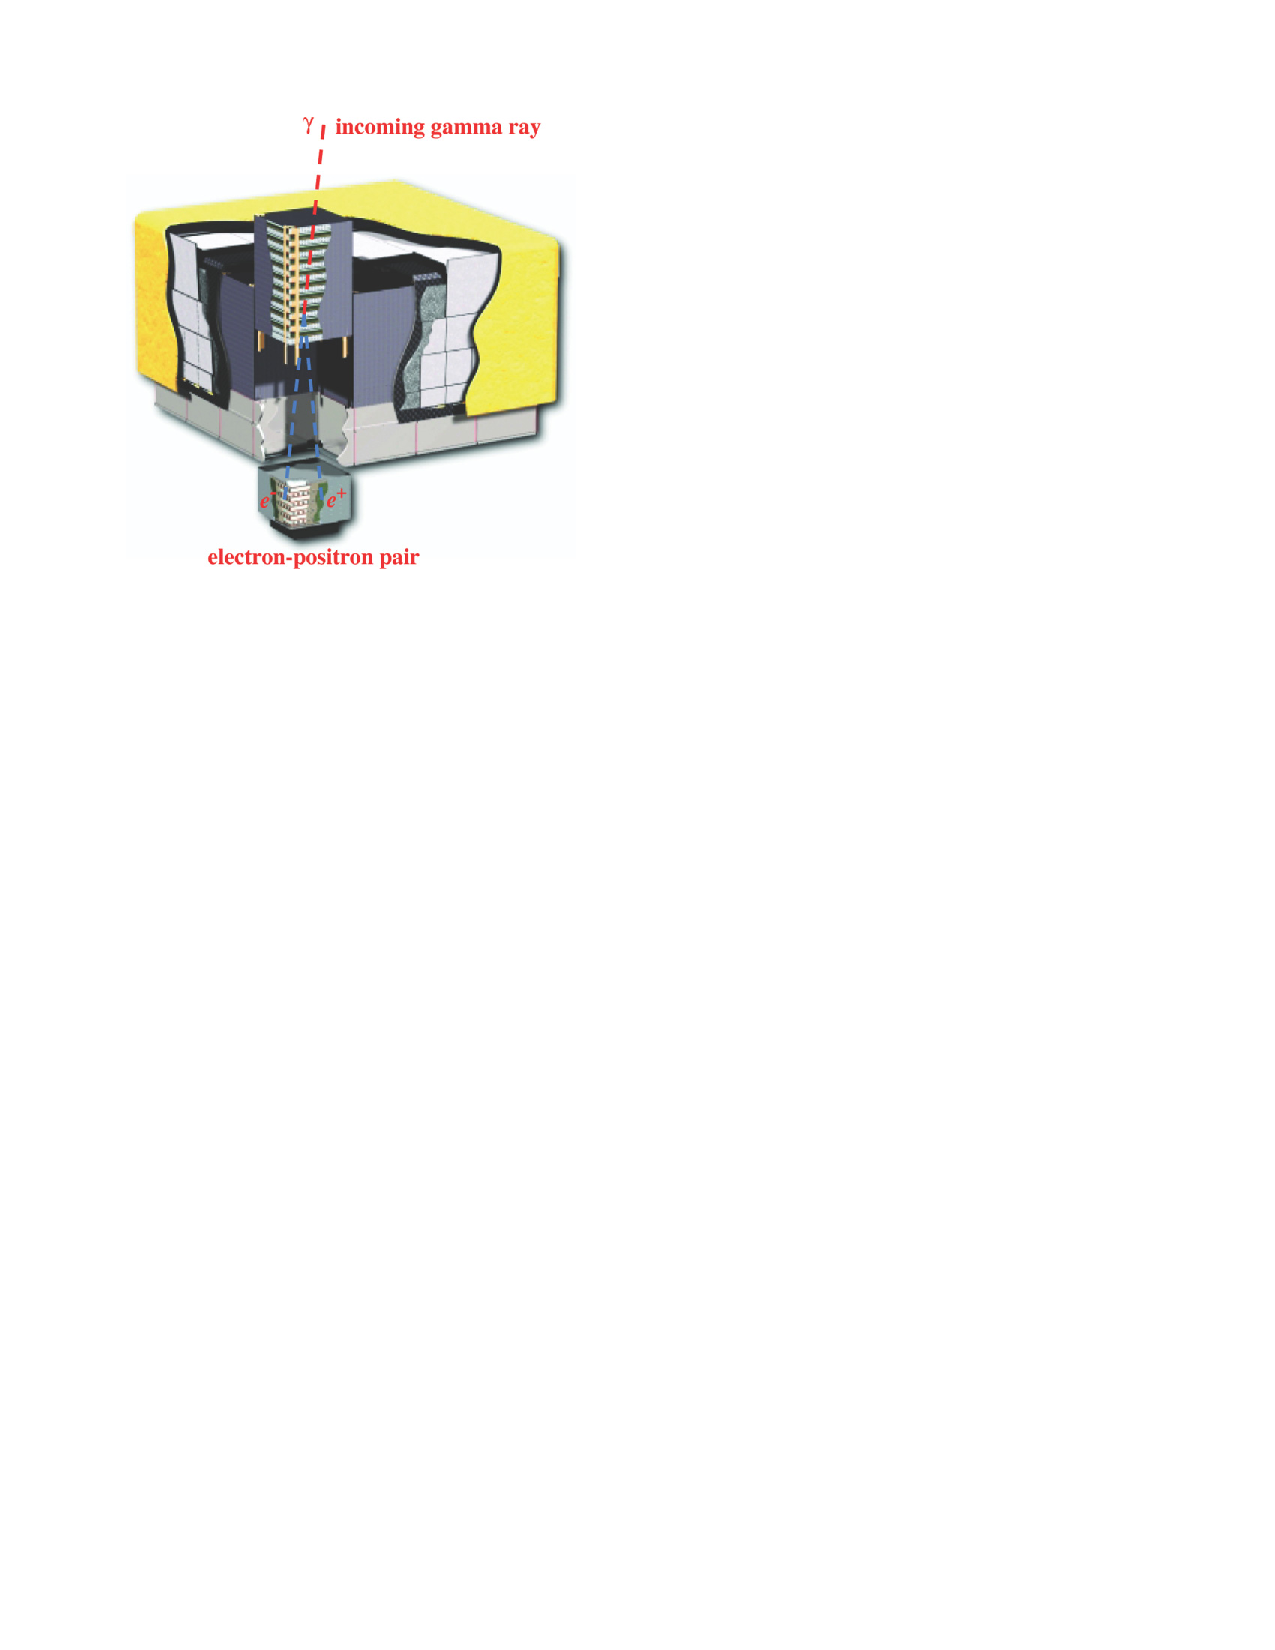
\includegraphics{chapters/introduction/figures/lat_detector_cutout.pdf}
  \caption{A schematic diagram of the \ac{LAT} with an incident
  $\gamma$-ray (red line) pair-converting into an electron
  and positron pair (blue lines).  This figure is taken from
  \citep{atwood_2009a_large-telescope}.}
  \figlabel{lat_detector_cutout}
\end{figure} 

The \fermi Gamma-ray Space telescope was launched on June 11, 2008 on
a Delta II heavy launch vehicle \citep{atwood_2009a_large-telescope}.
The primary since instrument on board \fermi is the \ac{LAT},
a pair-conversion telescope which detects $\gamma$-rays
in the energy range from $20\unitspace\mev$ to $>300\unitspace\gev$
(see \figref{lat_detector_cutout}).
In addition, \fermi contains the \Ac{GBM}, which is used to observe
\acp{GRB} in the energy range from $\sim8\unitspace\kev$ to $\sim40\unitspace\mev$.
See \cite{meegan_2009a_fermi-gamma-ray} for a description of the \ac{GBM}.

\subsection{The \acs{LAT} Detector}

The \ac{LAT} is composed of three major subsystems: the tracker, the
calorimeter, and the \ac{ACD}. Fundamentally, the detector operates by
inducing an incident $\gamma$-ray to pair convert in the tracker into
an electron and positron pair. The electron and position travel through
the tracker and into the \ac{CsI} calorimeter.  The tracks and energy
deposit can be used to infer the direction and energy of the incident
$\gamma$-ray.  Both the tracker and calorimeter are $4\times4$ arrays,
each composed of 16 modules.  Each tracker tower is divided into 18
tungsten converter layers and 16 dual-silicon tracker planes. Each
calorimeter module is composed of eight layers of 12 \ac{CsI} crystals.

The \ac{ACD} provides provides
background rejection of charged particles incident
on the \ac{LAT}.  The \ac{ACD} surrounds the tracker and is composed
of 89 plastic scintillator tiles ($5\times5$ on the top and 16
on each of the sides). The \ac{ACD} has a 0.9997 efficiency for
detecting singly-charged particles entering the \ac{LAT}.  A detailed
discussion of the various subsystems of the LAT can be found in
\citep{atwood_2009a_large-telescope}.

\subsection{Performance of the \acs{LAT}}
\subseclabel{performance_lat}

The \ac{LAT} 
has an unprecedented effective area ($\sim9,500\unitspace\cm^2$),
single-photon energy resolution ($\sim10\%$), and single-photon
angular resolution ($\sim3\fdg5$ at $\energy=100\unitspace\mev$
and decreasing to $\lesssim0\fdg15$ for $\energy>10\unitspace\gev$)
\citep{atwood_2009a_large-telescope}.

\begin{figure}[htbp]
  \centering
  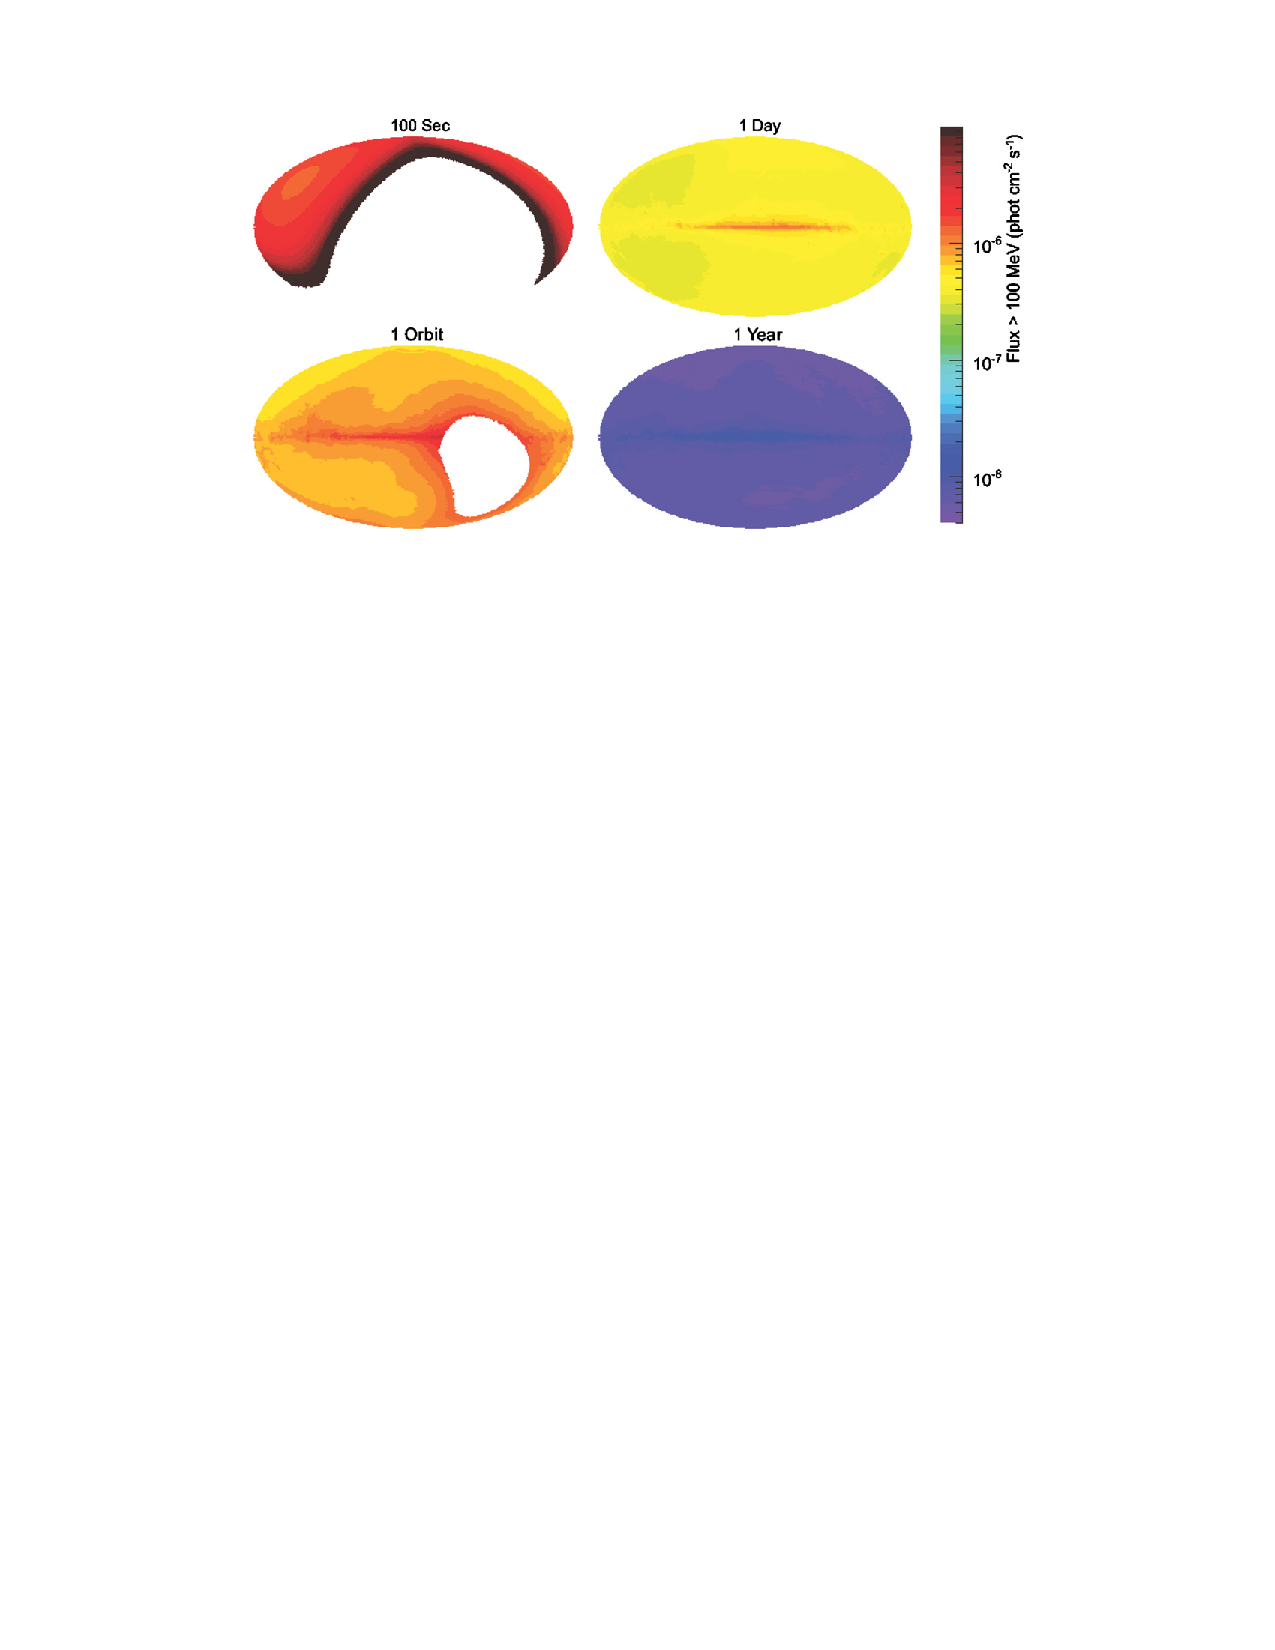
\includegraphics{chapters/introduction/figures/lat_point_source_sensitivity.pdf}
  \caption{
  The \ac{LAT} point-source sensitivity for exposures of
  $100\unitspace\second$, 1 orbit, $1\unitspace\dayunit$,
  and $1\unitspace\yearunit$.  This figure is from
  \cite{atwood_2009a_large-telescope}.
  }
  \figlabel{lat_point_source_sensitivity}
\end{figure} 

With its $2.4\unitspace\steradian$ field of view, \fermi can observe
the entire sky almost uniformly every $\sim3\unitspace\hour$.
With one year of observations, the \ac{LAT} has a point-source
flux sensitivity $3 \times 10^{-9} ($E>100\unitspace\mev$)
\ph\unitspace\cm^{-2}\second{-1}$ assuming a high-latitude diffuse
flux of $1.5\times10^{-5}\cm^{-2}\second^{-1}\steradian^{-1}$
($E>100\unitspace\mev$) \figref{lat_point_source_sensitivity} plots the
sensitivity for exposures of varying timescales.

\begin{figure}[htbp]
  \centering
  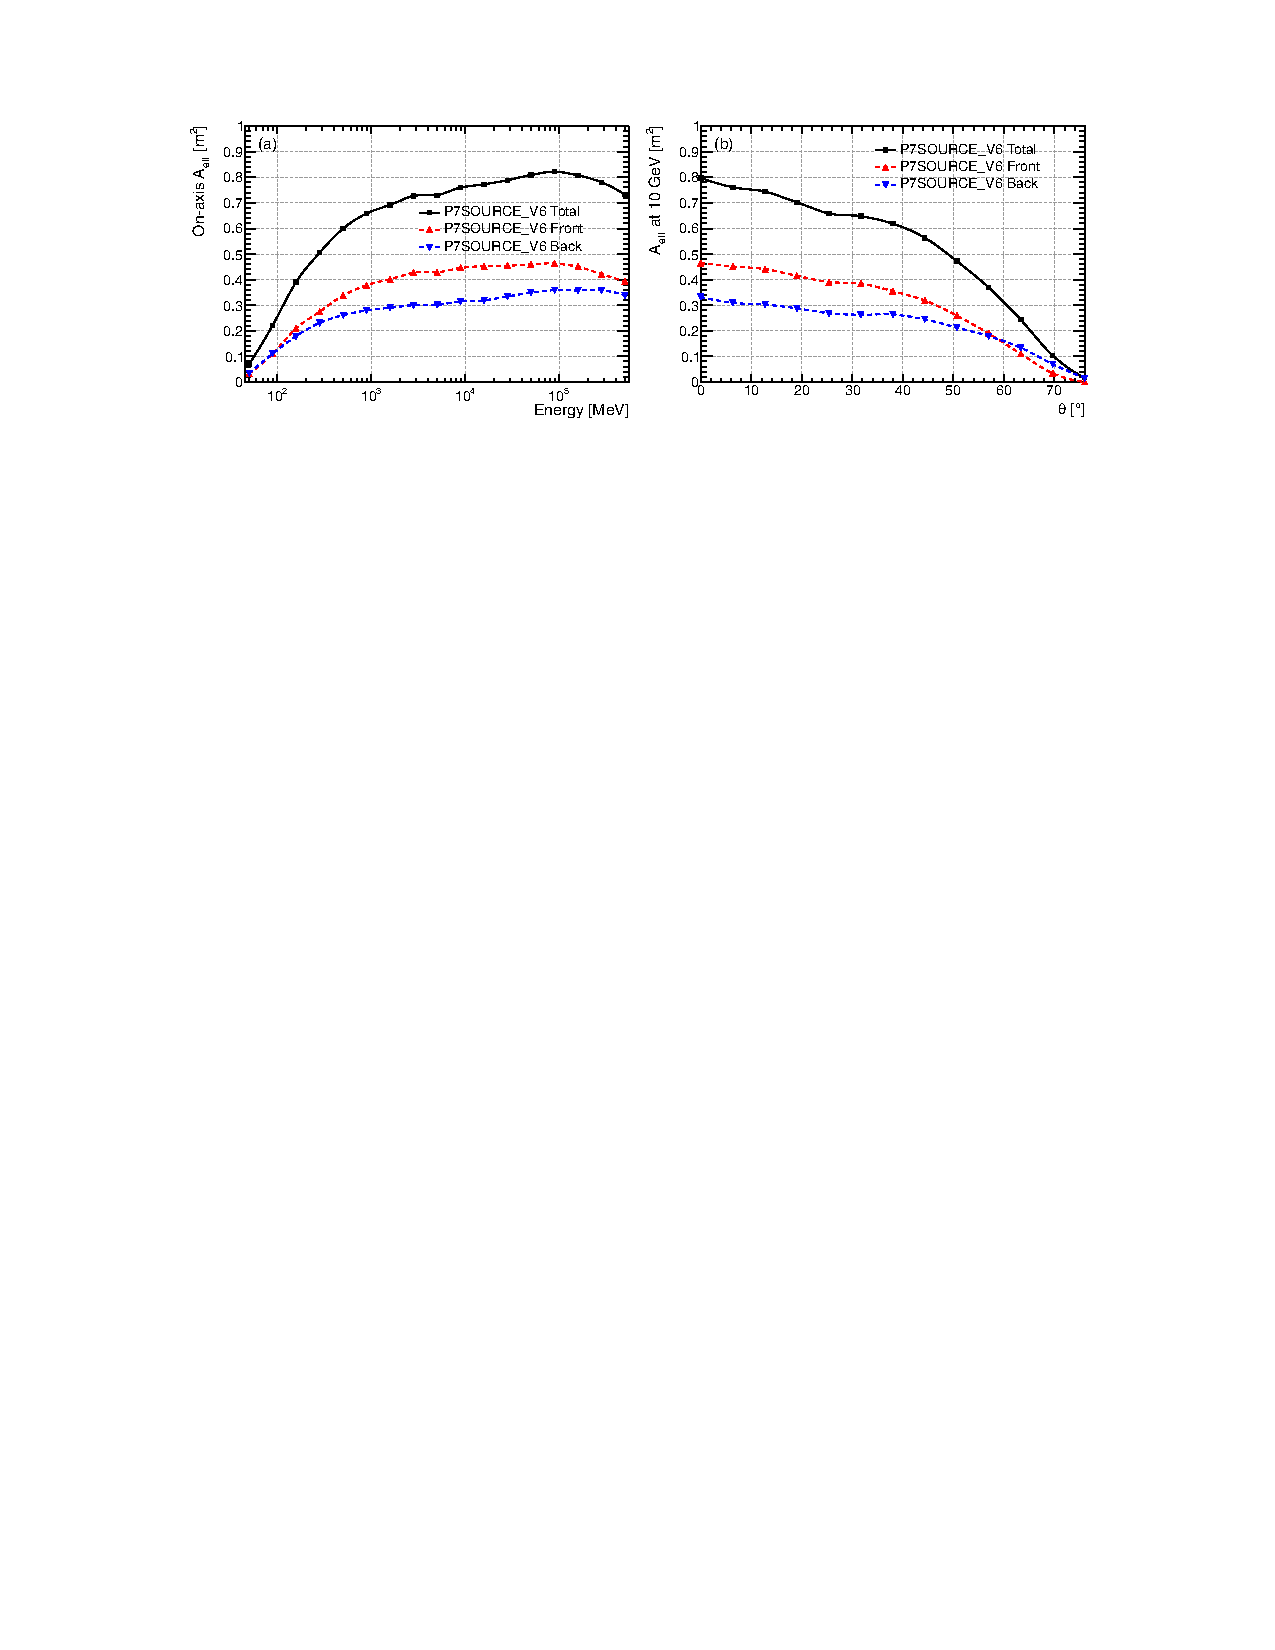
\includegraphics{chapters/introduction/figures/lat_effective_area.pdf}
  \caption{
  The \ac{LAT} effective area (a) as a function of energy for
  $\gamma$-rays that are incident on the \ac{LAT} perpendicularly from
  above and (b) as a function of incident angle for photons with an
  energy of $10\unitspace\gev$.  The \ac{LAT} performance is computed
  for the \psevensourcevsix event classification.  This figure is from
  \cite{ackermann_2012a_fermi-large}.
  }
  \figlabel{lat_effective_area}
\end{figure} 

\begin{figure}[htbp]
  \centering
  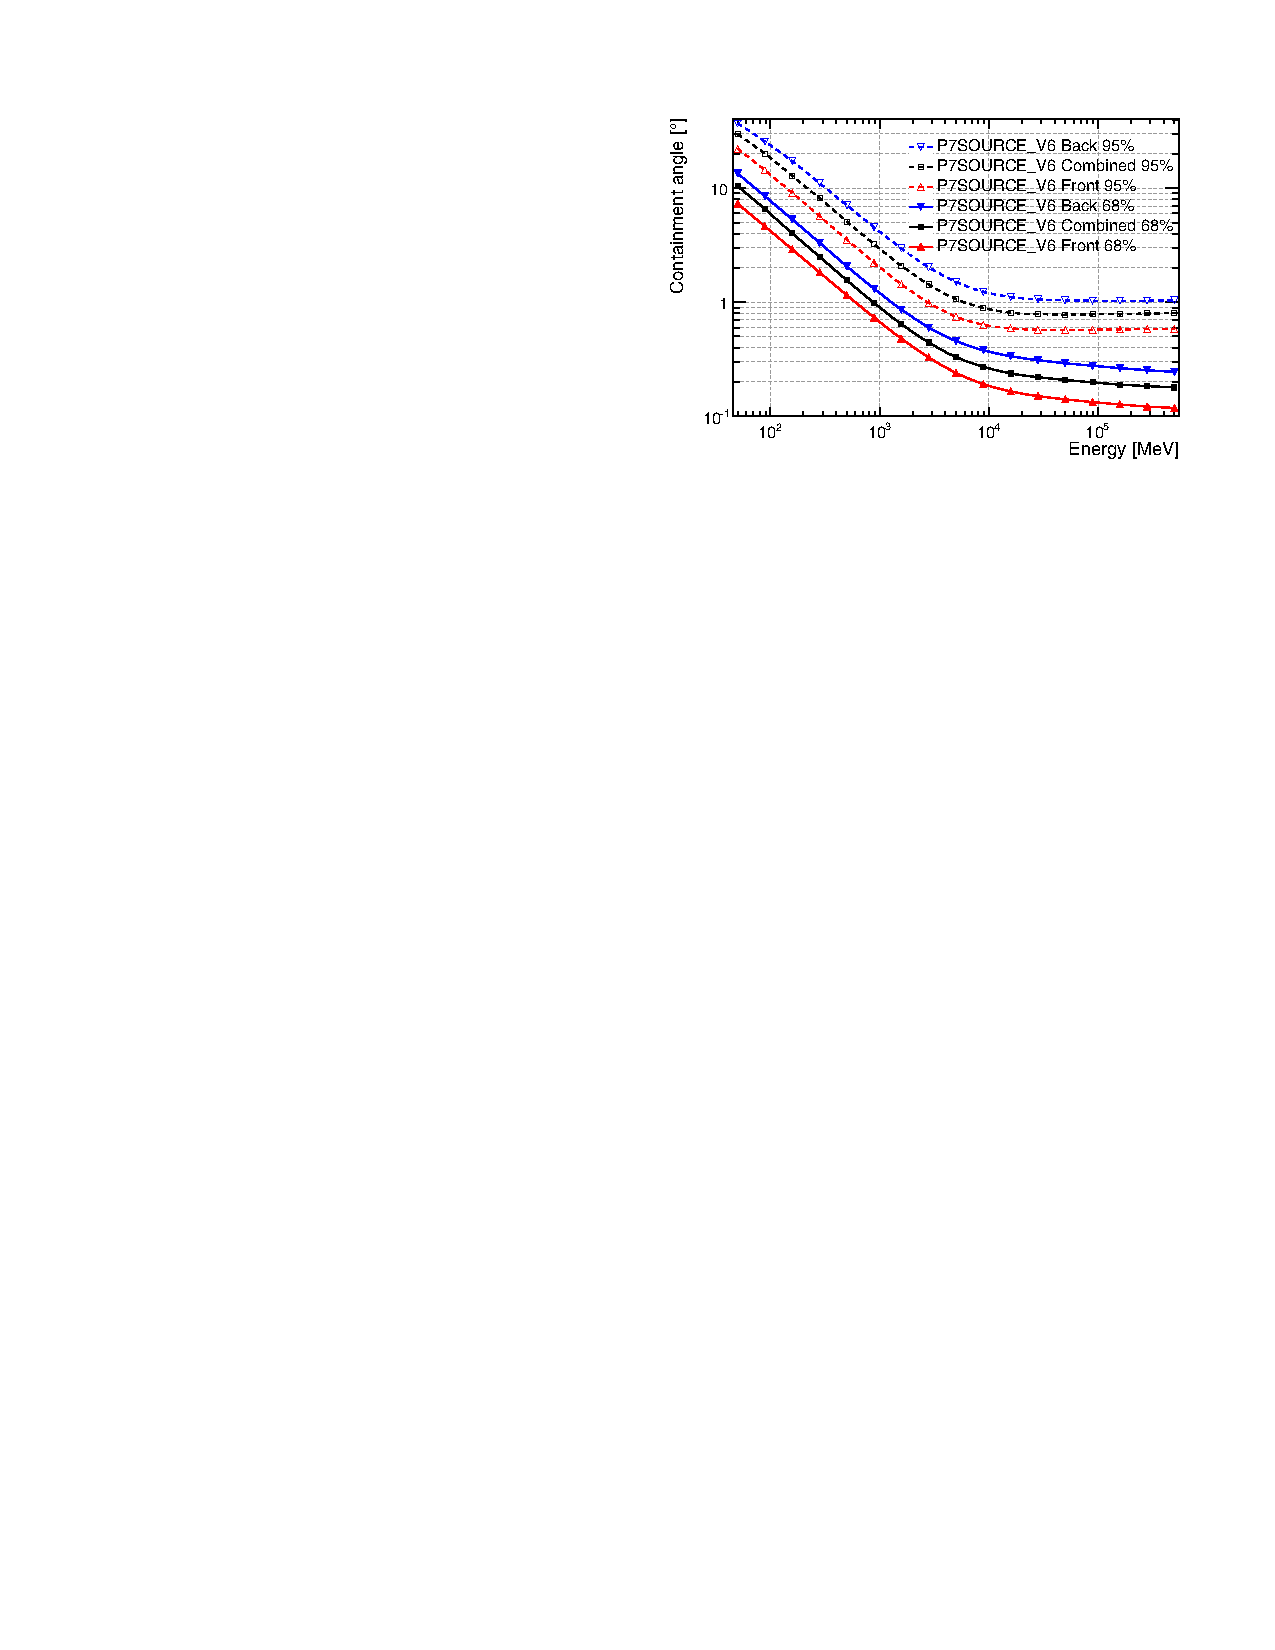
\includegraphics{chapters/introduction/figures/lat_psf.pdf}
  \caption{
  The angular resolution (68\% and 95\% containment radius)
  as a function of energy.
  The \ac{LAT} performance is computed for the \psevensourcevsix
  event classification.
  This figure is from \cite{ackermann_2012a_fermi-large}.
  }
  \figlabel{lat_psf}
\end{figure} 


\begin{figure}[htbp]
  \centering
  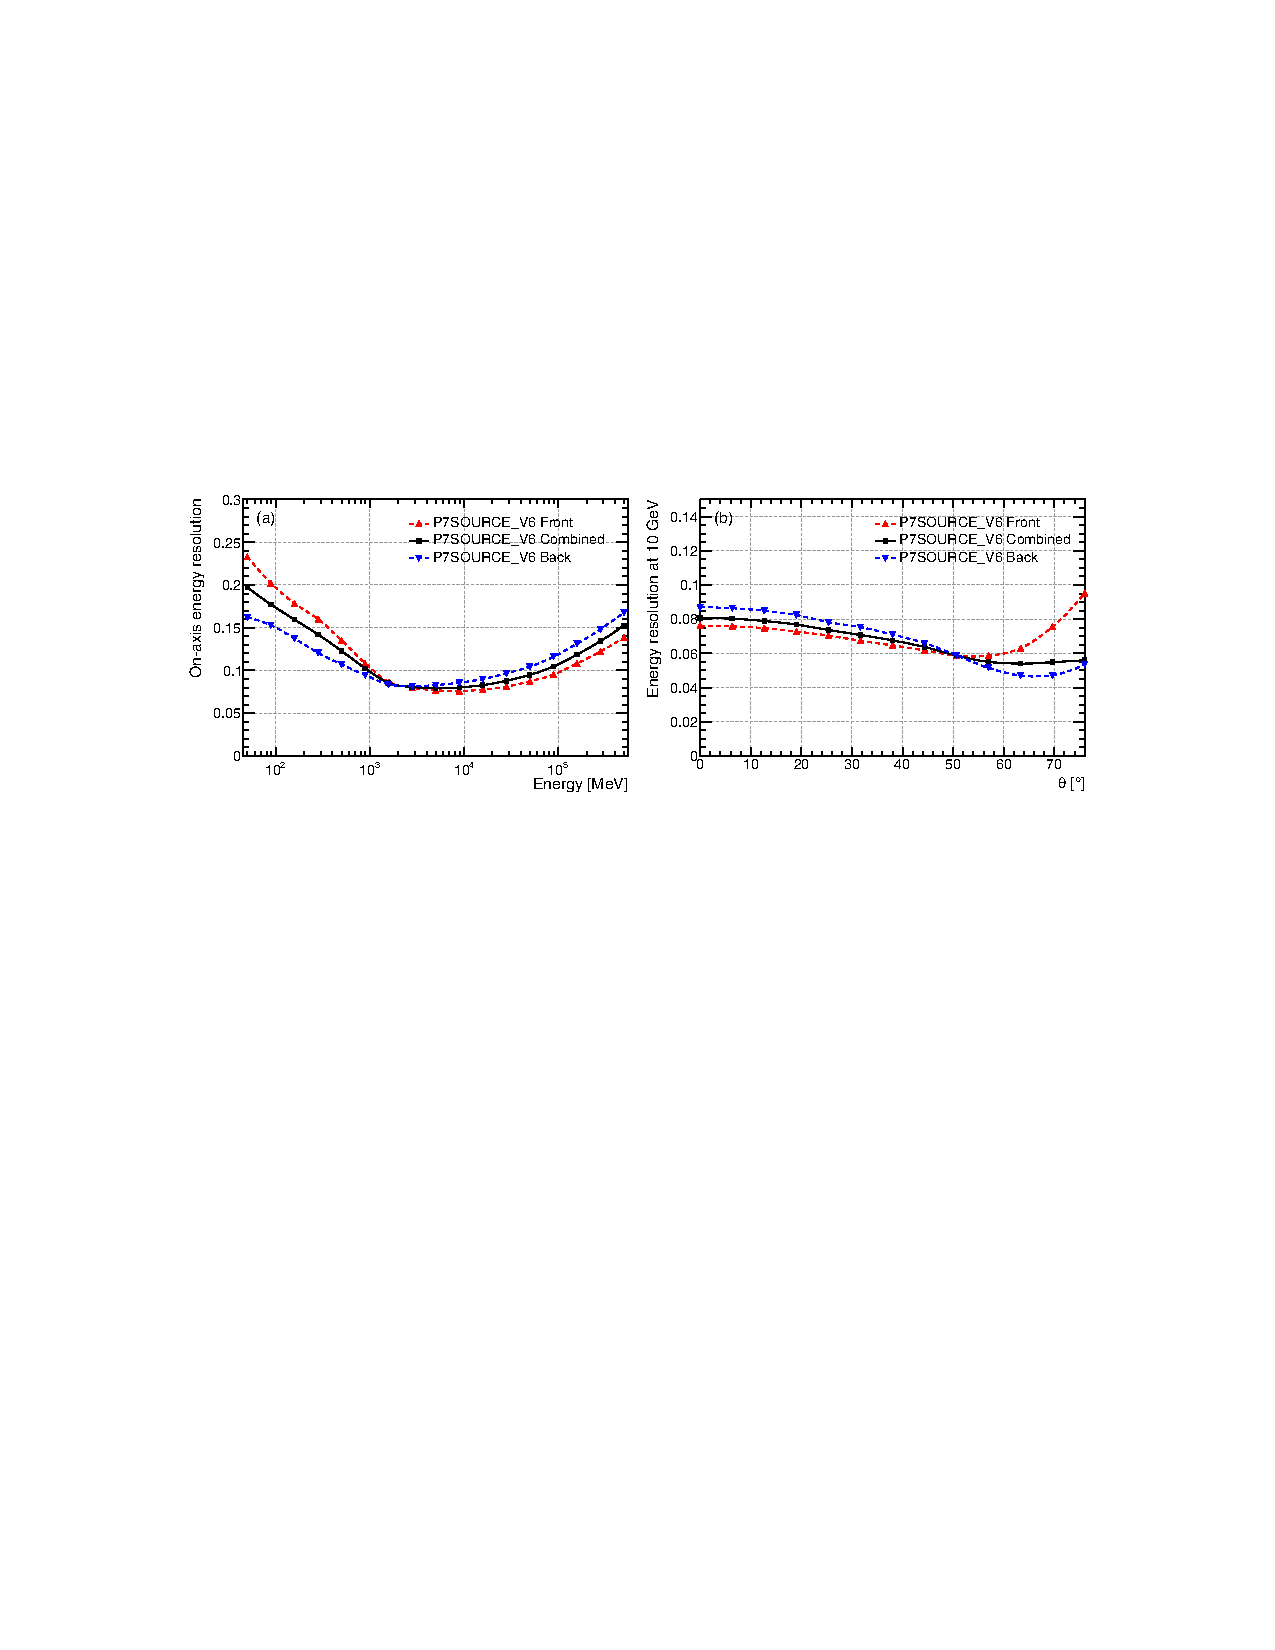
\includegraphics{chapters/introduction/figures/lat_energy_dispersion.pdf}
  \caption{
  The energy dispersion (a) as a function of energy for $\gamma$-rays that
  are incident on the \ac{LAT} perpendicularly from above and (b) as a function
  of the incident angle for photons with an energy of $10\unitspace\gev$.
  The \ac{LAT} performance is computed for the \psevensourcevsix
  event classification.
  This figure is from \cite{ackermann_2012a_fermi-large}.
  }
  \figlabel{lat_energy_dispersion}
\end{figure} 

The effective area, \ac{PSF}, and energy dispersion are both a function
of energy and of incident angle.  \figref{lat_effective_area} plots
the effective area as a function of energy and incident angle.
\figref{lat_psf} plots the \ac{PSF} as a function of energy.
Finally, \figref{lat_energy_dispersion} plots the energy dispersion
as a function of energy and incident angle.  We will describe in
\chapref{maximum_likelihood_analysis} the analysis methods used to
analyze \ac{LAT} data.
